\chapter[Introduction]%
{Introduction}

\section{The Occurrence of Ferroptosis}

The exploration of ferroptosis has unveiled a multitude of cellular factors and potential regulatory pathways. At its core, it is an intracellular, non-apoptotic, iron-dependent form of \ac{RCD} that is distinct from apoptosis, necrosis, and autophagy \citep{ferro_cd}. As the name suggests, this phenomenon is principally driven by iron molecules absorbed by cells from the surrounding extracellular environment. One such receptor is \ac{TFR1}, which mediates endocytosis of diferric transferrin \citep{tfr1}. This intracellular iron is often transported and stored in storage proteins such as ferritin, aiding in maintaining iron homeostasis and metabolism \citep{ferritin}.

Labile iron, however, which refers to loosely bound or chelatable iron, becomes a critical player in the ferroptotic process. Labile iron participates in the Fenton reaction, leading to the generation of \ac{ROS}, particularly hydroxyl radicals \citep{labile_iron}. \acs{ROS}, in turn, contributes to oxidative stress within the cell. 

\Acp{PUFA} in cellular membranes are highly susceptible to oxidative damage by \acs{ROS} \citep{lpperox}. Lipid peroxides are formed as a result of the oxidation of these fatty acids. Accumulation of lipid peroxides disrupts the integrity of cellular membranes, particularly the lipid bilayer \citep{lppmembrane}. Membrane damage leads to the loss of compartmentalization and function within the cell, including the mitochondrion \citep{lppmito}.

Healthy mammalian cells stave off this threat in a number of ways. The primary cellular mechanism of protection against oxytosis/ferroptosis is mediated by \ac{GPX4}, a glutathione-dependent hydroperoxidase that converts lipid peroxides into non-toxic lipid alcohols \citep{gpx4}. \ac{GSH} itself, which is produced from cysteine, is able to neutralize \acs{ROS} present within the cell directly, playing the role of antioxidant \citep{glutath}. 

Even when \acs{GPX4} functionality is uncompromised, research has shown that the mitochondrion plays a substantial role in ferroptosis regulation and induction, being the major compartment for cellular iron metabolism \citep{mito_ferro2}. Mitochondrial shrinkage and rupture are also common observations when a cell undergoes ferroptosis, since this organel is enveloped in a membrane \citep{mito_ferro}.

\begin{figure}[ht]
	\begin{center}
		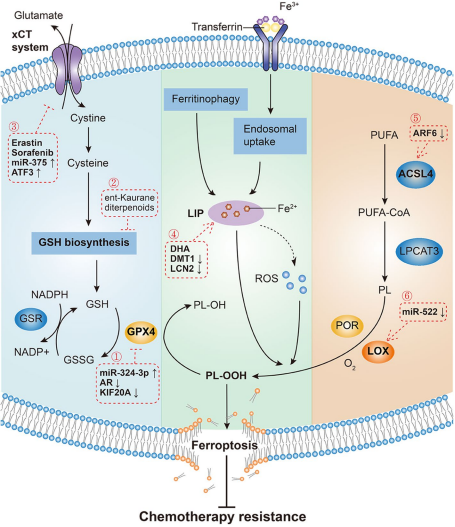
\includegraphics[width = 0.5\textwidth]{Fig/ferroptosis.png}
		\end{center}
		\caption{Figure depicting the various regulatory pathways associated with ferroptosis \citep{ferro_cancer}.}\label{fig:ferro_mech}
\end{figure}

\section{The Prospect of Ferroptosis in Cancer Therapy}

Cancer is the second leading cause of death worldwide, behind cardiovascular disease \citep{cancer}. However, improvements in cancer survival rates have occurred due to the increasing use of precision medicine or immunotherapy.

The prevalence of acquired resistance to targeted therapy underscores the urgent need for effective strategies to combat drug resistance. Recent findings highlight the significant role of ferroptosis in cancer therapy, disrupting target molecules and influencing cancer progression. Furthermore, studies have indicated that leveraging ferroptosis may offer a promising avenue to overcome resistance to targeted therapy \citep{ferro_drugs}.

Ferroptosis is commonly acknowledged as a tumor suppressor mechanism. Research has demonstrated that the inactivation of the p53 tumor suppression pathway, implicated in the genesis of most human cancers, is correlated with the suppression of ferroptosis \citep{p53}. Activation of p53 obstructs cystine uptake via the cystine/glutamate antiporter, thereby reducing intracellular \acs{GSH} levels and shielding tumor cells from ferroptosis. 

The synthesis and validation of ferroptosis inducers through various in vivo experiments underscore their potential as a viable anticancer therapy for clinical use pending extensive population validation. Consequently, numerous investigations have delved into the development of diverse inducers to trigger ferroptosis, examining its efficacy in various cancer treatment modalities including chemotherapy, immunotherapy, radiotherapy, nanotherapy, SDT, and PDT.

Tumor drug resistance arises from a multitude of mechanisms, with the disruption of redox homeostasis emerging as a pivotal factor. Tumor cells bolster their resilience against oxidative stress by curtailing their own production of acs{ROS}, fostering the development of acquired drug resistance \citep{ferro_res}.

\section{DNA Methylation and its Role in Cancer}

Mammalian DNA methylation primarily occurs as a covalent addition of methyl group to the carbon-5 atom of cytosine in a cytosine-guanine (CpG) dinucleotide. This enzymatic reaction is catalyzed by three DNA methyltransferases (DNMTs). DNMT3A and DNMT3B show equal preference to hemimethylated and unmethylated DNA molecules and are essential for the creation of initial DNA methylation marks (Okano et al. 1999). DNMT3A and DNMT3B are highly expressed in embryonic stem (ES) cells and, though downregulated, continue to be expressed in somatic cells (Sharma et al. 2011). After replication of the DNA, the newly synthesized strand does not carry the methylation modification. DNMT1 preferentially catalyzes the covalent addition of the methyl group onto the unmethylated strand of the hemimethylated DNA molecule. While DNMT1 carries out the majority of the DNA methylation in a dividing cell, DNMT3a/3b strongly associate with nucleosomes to permit efficient propagation of DNA methylation by modification of those sites missed by DNMT1 (Okano et al. 1999; Liang et al. 2002; Rhee et al. 2002; Jones and Liang 2009; Sharma et al. 2011).

DNMTs are responsible for laying down methyl groups, whereas the recently identified ten-eleven translocation (TET) family of dioxygenases provide a paradigm for DNA demethylation. These enzymes, through successive enzymatic reactions, can oxidize 5-methylcytosine (5mC) to 5-hydroxymethylcytosine (5hmC) and 5-formylcytosine (5fC) to 5-carboxylcytosine (5caC) (Ko et al. 2010; Pastor et al. 2011, 2013). The oxidization of 5mC contributes to the passive loss of DNA methylation over cell replication. In addition, the oxidized intermediates can be restored to cytosine by iterative oxidation followed by base excision repair mediated by thymine DNA glycosylase (TDG) (Kohli and Zhang 2013). Together, with DNMTs, these enzymes provide a model for the dynamic regulation of DNA methylation.

Methylated cytosine residues are susceptible to spontaneous deamination resulting in the poorly repaired cytosine to thymine transition. As a result, nearly a third of all disease-causing familial mutations and single-nucleotide polymorphisms are found in methylated CpG sites. Similarly, in somatic cells, CpG residues in the gene body or coding regions habitually contribute to mutational hot spots, such as in the case of inactivating C to T transitions at the tumor suppressor gene p53 (Pfeifer 2000; Jones and Baylin 2002).

Another consequence of this phenomenon is that there is a reduced representation of the CpG palindrome globally in the human genome, except in genomic regions designated as CpG islands (CGIs). CGIs were first defined by Gardiner-Garden and Frommer as a 200-bp DNA with a C + G content of 50 \% and an (observed CpG)/(expected CpG) in excess of 0.6 (Gardiner-Garden and Frommer 1987). While the majority of CpGs are methylated, CpG sites located in CGIs remain overwhelmingly unmethylated (Meissner et al. 2008). These islands are often, but not exclusively, found in the nearly half of all gene promoters (Mikkelsen et al. 2007; Meissner et al. 2008). Non-CGI promoters, on the other hand, are predominantly methylated and silent. These genes are more likely to be tissue specifically expressed; therefore, only a small subset of non-CGI promoters remain unmethylated and accessible for transcription factors in each tissue type (Eckhardt et al. 2006).

Recent advancements in next-generation sequencing techniques applied to cancer genomes have unveiled a prevalent pattern of mutations recurring in diverse epigenetic modulators. These modulators encompass mediators of DNA methylation, covalent histone modifiers, and genes encoding subunits of chromatin remodelers \citep{meth_cancer}. The aberrant functioning of these pivotal epigenetic regulators leads to the dysregulation of gene expression and is implicated in a myriad of malignancies, spanning various cancer types \citep{meth_cancer2}.

\section{DNA Methylation Detection Techniques}

Bisulfite genomic sequencing stands as the benchmark technology for detecting DNA methylation due to its ability to offer qualitative, quantitative, and highly efficient insights into identifying 5-methylcytosine at single base-pair resolution. Initially pioneered by \cite{bisulfite_ori}, this method capitalizes on the discovery that the amination reactions of cytosine and \ac{5mC} yield markedly distinct outcomes following treatment with sodium bisulfite.

In this context, cytosines present in single-stranded DNA undergo conversion into uracil residues, which are subsequently recognized as thymine during PCR amplification and sequencing. However, \acsp{5mC} remain unaffected by this conversion, retaining their cytosine identity and enabling the distinction between methylated and unmethylated cytosines \citep{bisulfite2}. 

Following bisulfite treatment, a subsequent PCR step becomes imperative to ascertain the methylation status at specific loci, employing methylation-specific primers. The actual methylation status can then be determined through either direct sequencing of PCR products (for the detection of average methylation status) or sub-cloning sequencing (for the detection of the distribution of methylation patterns at the single-molecule level) \citep{bisulfite2}.

Despite being the current gold standard, bisulfite sequencing is not without its flaws. Understanding bisulfite-treated DNA data requires careful consideration of two types of conversion errors: failed conversion and inappropriate conversion. Failed conversion, extensively studied, arises when an unmethylated cytosine fails to deaminate, resulting in its appearance as methylated in sequencing data. In mammalian somatic cells, where 5-methylcytosine primarily occurs at CpG cytosines, the frequency of failed conversion is indicated by the proportion of non-CpG cytosines appearing as cytosines in sequence data \citep{bisulfite_failed_conv}. Ignoring failed conversion in data analysis can inflate methylation density estimates and impede the determination of DNA methyltransferase sequence motif preferences.

Inappropriate conversion, the second type of error, occurs when a methylated cytosine undergoes deamination, yielding thymine \citep{bisulfite_inappr_conv}. Similar to uracils resulting from cytosine deamination, thymine pairs with adenine during PCR. Consequently, 5-methylcytosines subjected to inappropriate conversion are misinterpreted as unmethylated. Failure to account for inappropriate conversion leads to underestimation of genomic methylation densities. However, if the frequency of inappropriate conversion is known, it can be integrated as a parameter in data analysis. Therefore, information on both failed and inappropriate conversion frequencies is crucial for drawing meaningful insights from detailed DNA methylation patterns.

In addressing the limitations of bisulfite sequencing, new techniques have emerged despite its status as the gold standard for detecting methylation marks. These limitations encompass the aforementioned confounding effects of bisulfite treatment on DNA methylation, alongside the challenge of distinguishing between DNA methylation and hydroxylation \citep{ont_vs_bisulfite}. In light of these considerations, we advocate for the utilization of Nanopore sequencing as a promising alternative for identifying methylation marks.

Nanopore sequencing is a next-generation sequencing technology that enables the real-time analysis of DNA or RNA molecules as they pass through a nanoscale pore. This technique is based on the principle that as a DNA strand translocates through a nanopore, changes in the electrical current can be measured and used to deduce the sequence of the DNA molecule \cite{ont}. 

The raw electrical signal is translated into DNA sequence information through a process called basecalling. DNA methylation involves the addition of a methyl group to a cytosine base, commonly referred to as a 5-methylcytosine. Nanopore sequencing can detect these modifications as changes in the electrical current during translocation using specialized algorithms and basecallers (Fig. \ref{ont_epi}).

\begin{figure}[ht]
	\begin{center}
		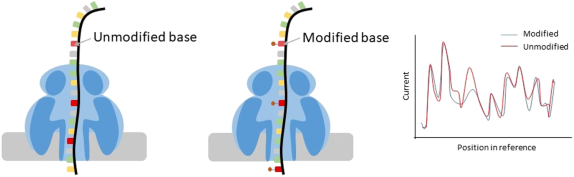
\includegraphics[width = \textwidth]{Fig/ont_epi.png}
	\end{center}
	\caption{Direct base modification detection with \acs{ONT}.}\label{ont_epi}
\end{figure}

One of the key advantages of nanopore sequencing is its ability to generate long reads, providing information about entire genomic regions in a single continuous sequence. Short-read sequencing offers a cost-effective and accurate solution, bolstered by a diverse array of analysis tools and pipelines \citep{short_reads}. However, the vast range of lengths spanning natural nucleic acid polymers, extending over eight orders of magnitude, presents a challenge when sequencing them in short amplified fragments, hindering the reconstruction and quantification of the original molecules. 

Long reads, on the other hand, hold the potential to enhance de novo assembly, ensure mapping accuracy, facilitate transcript isoform identification, and enable the detection of structural variants. Moreover, the sequencing of native molecules, both DNA and RNA, using long reads, eliminates amplification bias while retaining base modifications \citep{long_read_adv}. These capabilities, coupled with ongoing advancements in accuracy, throughput, and cost reduction, are establishing long-read sequencing as a viable option for a wide spectrum of genomic applications in both model and non-model organisms \citep{long_read_adv2}.

Adaptive sampling is a feature that helps optimize the sequencing process by adjusting data collection parameters in real-time based on the characteristics of the DNA being sequenced. The system monitors various parameters such as the quality of the signal, the speed at which the DNA is translocating through the nanopore, and other relevant metrics \citep{ont_as}. The software requires a user to upload a file of whitelisted reference sequences, and the system can be set to either deplete or enrich for these on a specified set of channels. 

In order to achieve this, the software basecalls the first few hundred bases of each read and compares it with the target reference sequences. Matching or unmatching sequences are rejected, depending on whether the software is set to enrich or deplete. By using this, coverage of our genes of interest is enriched, greatly reducing noise.